\section{Systematic Literature Review}
We applied a two-step research approach, whereby we first conducted a systematic literature review to identify relevant publications before analysing the identified publications for the coding of benefits and directions. After coding, we grouped all found benefits. This process is illustrated in \ref{fig:ResearchApproachGathering} for data collection and in \ref{fig:ResearchApproachAnalysis} for data analysis.

\subsection{Data Collection}
For the identification of papers addressing Augmented Reality in educational environments, we applied a systematic online literature database search. We included databases which were specialised on more information systems centered papers, namely Institute of Electrical and Electronic Engineers (IEEE) Xplore Digital Library, ProQuest (ABI / INFORM), Association for Information Systems Electronic Library (AISel) and Association for Computing Machinery (ACM) Digital Library, as well as more general databases, namely EBSCO Host and ScienceDirect.\\
To find relevant papers, we searched within all databases with on the following attributes: title, abstract and author supplied keywords. Within these keywords we had three mandatory groups of keywords. Every article had to include the keyword "Augmented Reality". Additionally, every article needed to have at least one synonym for education and benefits. Namely we searched for "Educat*", "Learn*", "Teach*", "College" or "School" as synonyms for education and "Benefi*", "Advan*", "Improv*", "Enhanc*", "Driver*" or "Value*" as synonyms for benefits. To deal with the limitations of some databases, we had to split our query and conduct multiple queries on the database and merge them together by hand.\\
This database query resulted in a total of 523 articles. Those results were checked against our include- and exclude-criteria, which are listed in \ref{tab:IncludeExcludeCriteria}, and were preliminary coded into one of the five directions. This process was performed by ourselves and each article was read by two of the authors.\\
After merging our results, a total of 25 articles remained.

\begin{figure}[ptbh]
    \centering
    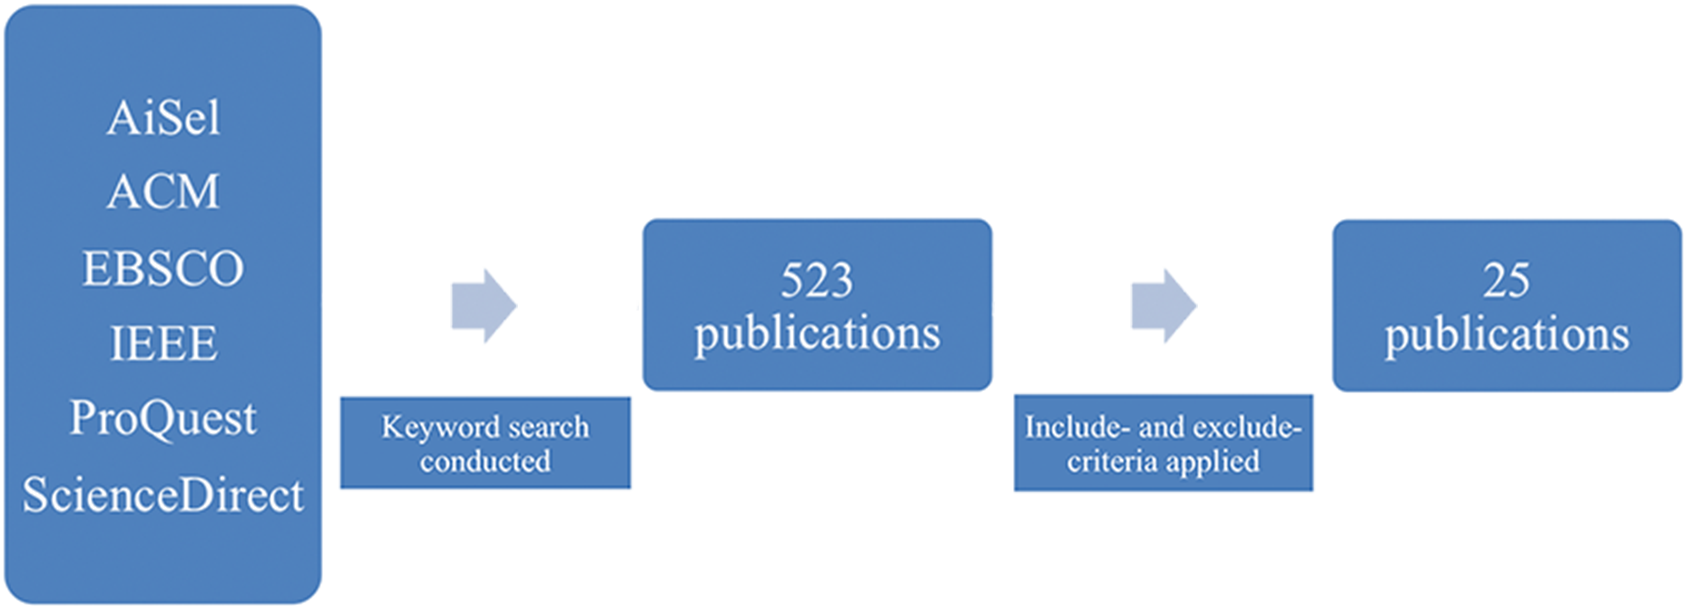
\includegraphics[width=\linewidth]{figures/research_approach_part_1.png}
    \caption[Research Approach: Data Gathering]{Research Approach: Data Gathering}
    \label{fig:ResearchApproachGathering}
\end{figure}

\begin{figure}[ptbh]
    \centering
    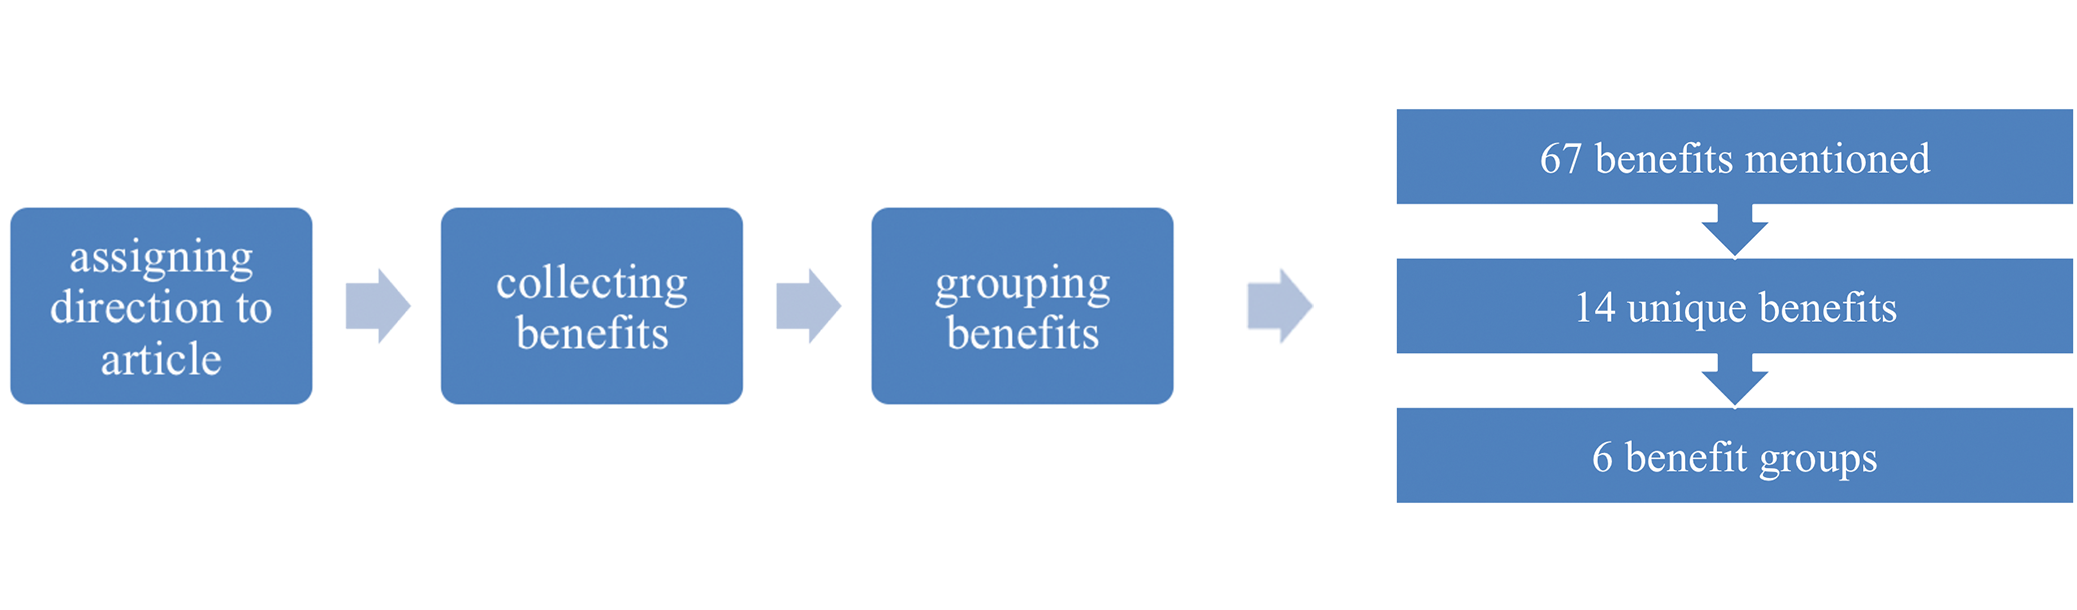
\includegraphics[width=\linewidth]{figures/research_approach_part_2.png}
    \caption[Research Approach: Data Analysis]{Research Approach: Data Analysis}
    \label{fig:ResearchApproachAnalysis}
\end{figure}

\begin{table}[ptbh]
    \center
    \vspace{1em}
    \begin{tabular}{p{17em} | p{17em}}
        \textbf{Include Criteria} & \textbf{Exclude Criteria} \\
        \hline
        Empirical works & theoretical works, grey literature, dissertations \\
        A teaching problem is solved with the help of Augmented Reality or a teaching concept is improved by Augmented Reality & untried or untested technologies, concepts without empirical evidence \\
        Lists positive effects of Augmented Reality applications in comparison to conventional learning tools & No control-group or control-scenario provided, no comparison to conventional learning tools \\
        Human learning & Machine learning \\
        English language & Other language \\
        Peer-reviewed & not peer-reviewed \\
    \end{tabular}
    \caption[Include- and Exclude-Criteria]{Include- and Exclude-Criteria}
    \label{tab:IncludeExcludeCriteria}
\end{table}

\subsection{Data Analysis}
During data analysis we grouped all found benefits into major groups and matched all found benefits to the directions of the articles in which they were mentioned. We will go into details regarding the benefits found and the grouping of them in chapter \ref{subsec:Benefits} and regarding the mapping of benefits to directions in chapter \ref{subsec:Mapping}.\\
Because of our orientation towards the five directions, we assigned directions to all articles during data collection but revised our assignment in case of differences between the first and second coder. Our inter coder reliability score is 0.64. We will interpret and discuss this score in chapter \ref{sec:Discussion}. During assignment of directions we also collected all mentioned benefits and generalised similar benefits into a single one. Afterwards, those benefits were grouped into broader topic-related benefits.\\
A total of 67 benefits were mentioned, containing 14 unique benefits, which were grouped into six groups.